% \documentclass{article}
\documentclass[fleqn]{article}
\usepackage{amsmath}
\usepackage{enumitem}
\usepackage{import}
\subimport*{../assignment-2/}{macro}

\setlength\parindent{20px}
\setlength{\mathindent}{20pt}

\begin{document}
\title{Homework \#4}
\author{Aaron Chen / aaronyc}
\date{}
\maketitle

% ------ setting ------

\subsection*{A1. Conceptual Questions}

\begin{enumerate}[label=(\alph*)]
\item
True. Since $\mathrm{rank}(X) = k$, all rows of $X$ lie in a $k$-dimensional subspace, and the top-$k$ principal components of PCA span exactly this subspace. Projecting onto it loses no information, so the reconstruction error is zero.

\item
False. From $X = USV^\top$, we have $X^\top X = V S^\top U^\top U S V^\top = V S^2 V^\top$, which is the eigendecomposition of $X^\top X$. This means the \emph{columns} of $V$, not the rows, are the eigenvectors of $X^\top X$ (with eigenvalues $\sigma_i^2$).

\item
False. The objective is monotonically non-increasing in $k$ and equals $0$ at $k = n$ (each point in its own cluster), so minimizing it trivially picks $k = n$, which gives no meaningful clusters.

\item
False. SVD is only unique up to sign flips of paired columns $(u_i, v_i)$, and to orthogonal rotations within subspaces corresponding to repeated singular values.

\item
False. The identity matrix $I_n$ has rank $n$ but only one unique nonzero eigenvalue ($\lambda = 1$ with multiplicity $n$).
\end{enumerate}

% ---------------------

\subsection*{A2. Think Before You Train}

\begin{enumerate}[label=(\alph*)]
\item
Preprocessing: handle missing values, one-hot encode categorical features, standardize numerical features, and address class imbalance with resampling or class-weighted loss. To deal with limited new-user input, I would use $k$-NN imputation to borrow richer feature values from the most similar training users. I would compare two predictors: L1-regularized logistic regression, whose sparse coefficients directly rank risk factors and need few samples, versus a small MLP, which captures nonlinear interactions but is hard to interpret and prone to overfitting. Since the institute wants to learn which factors matter most, I would deploy the L1 logistic regression and keep the MLP as an accuracy benchmark.

\item
Three shortcomings can yield different accuracy across populations:
\begin{itemize}
\item \textbf{Population and class imbalance}: underrepresented demographics and rare disease-positive cases pull the model toward the majority pattern. \emph{Fix:} stratified sampling, demographic reweighting, or class-weighted loss, and report per-subgroup accuracy.

\item \textbf{$k$-NN imputation failure}: minority users have few truly similar neighbors, so $k$-NN borrows feature values from dissimilar users. \emph{Fix:} add a distance threshold, restrict neighbors to the same stratum, or replace $k$-NN with a per-stratum parametric imputer.

\item \textbf{MLP interpretability gap}: entangled weights hide which features drive errors in specific subgroups, making fairness audits hard. \emph{Fix:} deploy the L1 logistic regression, or apply permutation importance and per-subgroup evaluation if the MLP is used.
\end{itemize}

\item
Ignoring these biases lets the model treat policing intensity and reporting rates as ground-truth crime, embedding existing inequities into the predictions. The main harm is a feedback loop: the model labels over-policed minority neighborhoods as high-crime, more police are sent there, more arrests are recorded, and the next round of training reinforces the prior. This also drives resource misallocation, since policing concentrates where the model predicts risk while social services and infrastructure investment are pulled away. Because the underlying biases fall disproportionately on minority communities, these harms accumulate on already disadvantaged populations.
\end{enumerate}

% ---------------------

\subsection*{A3. Image Classification on CIFAR-10}

\begin{enumerate}[label=(\alph*)]
\item
Search method: grid search over 5 configurations of hidden size $M$, learning rate, and momentum, trained for 20 epochs with SGD.

\begin{center}
\begin{tabular}{c|c|c|c}
Config & $M$ & lr & momentum \\
\hline
1 & $256$  & $0.01$  & $0.9$ \\
2 & $512$  & $0.01$  & $0.9$ \\
3 & $512$  & $0.005$ & $0.9$ \\
4 & $1024$ & $0.01$  & $0.9$ \\
5 & $1024$ & $0.005$ & $0.9$ \\
\end{tabular}
\end{center}

Best hyperparameters: $M = 512$, $\text{lr} = 0.01$, $\text{momentum} = 0.9$.

\[
\text{Test accuracy} = 0.4854
\]

\begin{center}
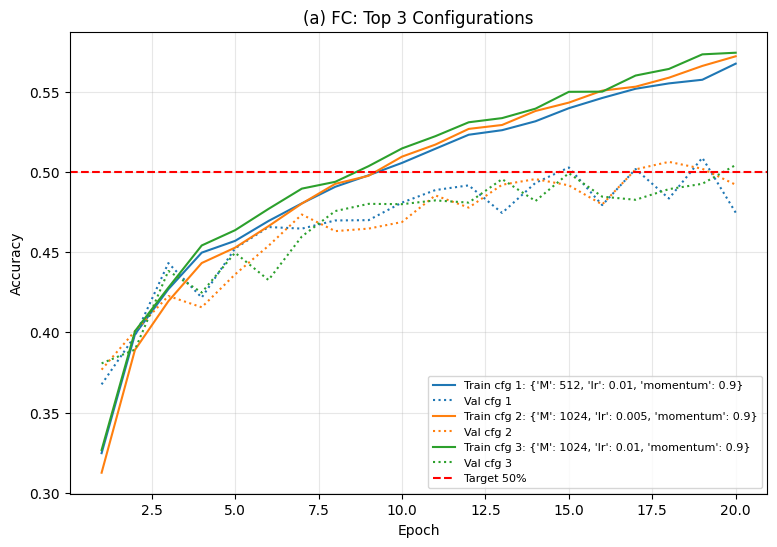
\includegraphics[width=0.8\textwidth]{hw4-A/cifar_fc_accuracy.png}
\end{center}

\item
Search method: grid search over 5 configurations of filter count $M$, filter size $k$, pool size $N$, learning rate, and momentum, trained for 20 epochs with SGD.

\begin{center}
\begin{tabular}{c|c|c|c|c|c}
Config & $M$ & $k$ & $N$ & lr & momentum \\
\hline
1 & $64$  & $5$ & $14$ & $0.01$  & $0.9$ \\
2 & $100$ & $5$ & $14$ & $0.01$  & $0.9$ \\
3 & $100$ & $5$ & $14$ & $0.005$ & $0.9$ \\
4 & $200$ & $5$ & $14$ & $0.01$  & $0.9$ \\
5 & $100$ & $7$ & $13$ & $0.01$  & $0.9$ \\
\end{tabular}
\end{center}

Best hyperparameters: $M = 200$, $k = 5$, $N = 14$, $\text{lr} = 0.01$, $\text{momentum} = 0.9$.

\[
\text{Test accuracy} = 0.6209
\]

\begin{center}
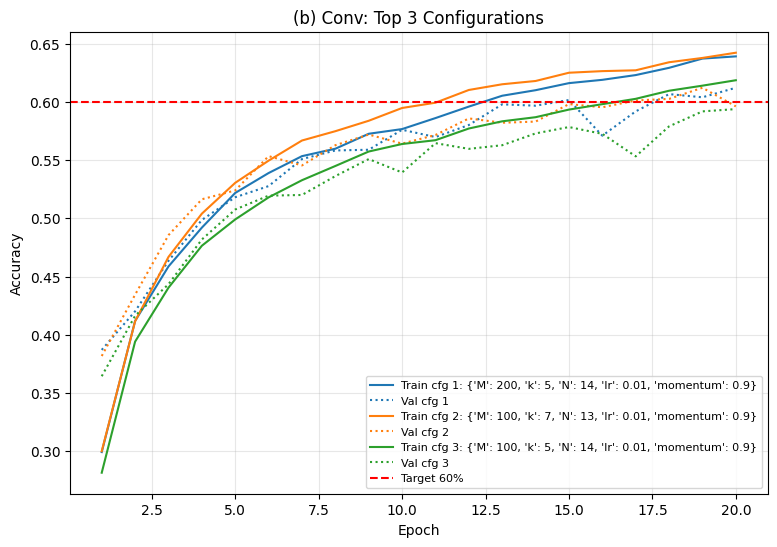
\includegraphics[width=0.8\textwidth]{hw4-A/cifar_conv_accuracy.png}
\end{center}
\end{enumerate}

% ---------------------

\subsection*{A4. $k$-means Clustering}

\begin{enumerate}[label=(\alph*)]
\setcounter{enumi}{1}
\item
\begin{center}
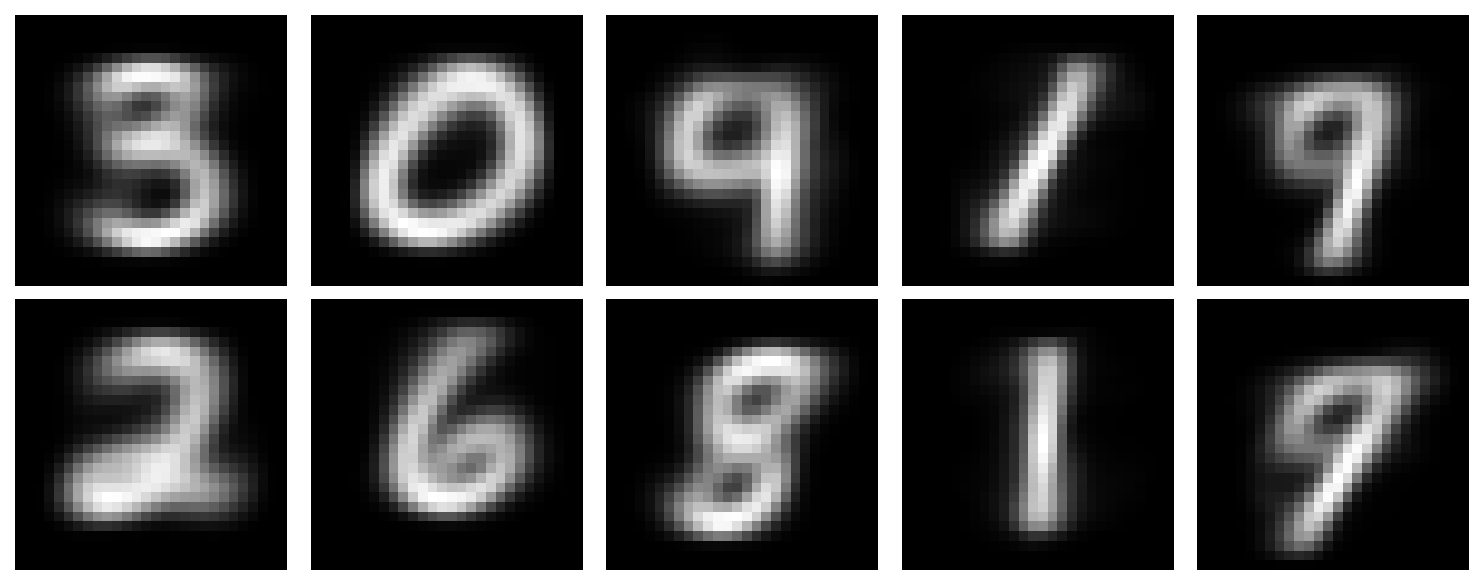
\includegraphics[width=0.8\textwidth]{hw4-A/kmeans_centers.png}
\end{center}
\end{enumerate}

% ---------------------

\subsection*{A5. Transformers}

\begin{enumerate}[label=(\alph*)]
\item
Training and validation loss curves:
\begin{center}
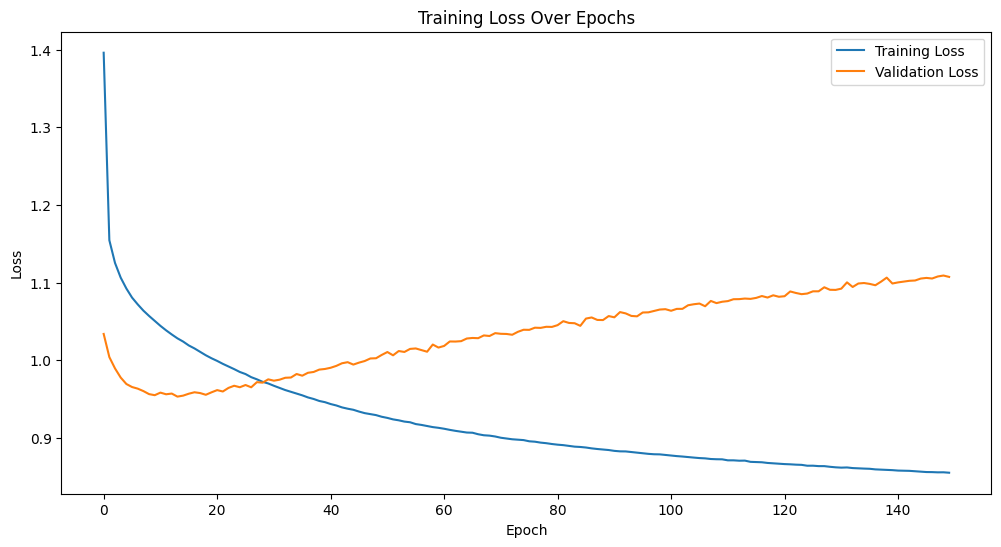
\includegraphics[width=0.8\textwidth]{hw4-A/transformer_loss.png}
\end{center}

Three example text generations:
\begin{itemize}
\item Prompt \texttt{<START>}:
\texttt{AUFIDIUS : My sorrows <UNK> : thy share amongst do not I ! <STOP>}

\item Prompt \texttt{KING RICHARD}:
\texttt{KING RICHARD <UNK> RICHARD <UNK> : Renowned I With below ; let the knight out of prison , That can not brook the}

\item Prompt \texttt{To be or not}:
\texttt{To be or not for all to shrink a noble York : and I send you , take a messenger , Repair he see}
\end{itemize}

\item
% Softmax sampling temperature T.
\begin{enumerate}[label=(\roman*)]
\item
$T \to 0^+$. As $T$ approaches $0$, the largest logit dominates the others after dividing by $T$, so the softmax collapses to a one-hot distribution on $\arg\max_i x_i$, which is exactly greedy decoding.

\item
$T = 1$. Setting $T = 1$ makes $x_i / T = x_i$, which recovers the standard softmax with no temperature scaling.

\item
$T \to \infty$. As $T$ grows, every $x_i / T \to 0$, so $e^{x_i / T} \to 1$ for all $i$, and the resulting distribution becomes uniform $1/n$ over the vocabulary.
\end{enumerate}

% \item
% Extra credit: transformer trained on personal email corpus.
\end{enumerate}

% ---------------------

% Reminder: Because AI help was used, include the required transcript with the submission.

% ------ setting ------

\end{document}
